\subsubsection{Dise\~no inicial de interfaz para control y monitorear}
    Para el dise\~no de la interfaz en la cual se puede controlar y a
        su vez, hacer uso del sistema de monitoreo del robot, es
        necesario conocer cada uno de los componentes que son
        necesarios mostrar y los que ser\'an necesarios para realizar la
        funcionalidad correspondiente, los cuales corresponden a los
        siguientes:
    \vskip 0.5cm
    Sistema de monitoreo: La interfaz debe mostrar la visi\'on de
        la c\'amara que esta incorporada al robot, por lo que debe de
        haber un espacio dedicado a mostrar a esta misma.
        \vskip 0.5cm
    Sistema LiDAR: En la interfaz tambi\'en se debe mostrar cada
        uno de los puntos que son obtenidos a trav\'es de este sistema,
        los cuales representan los obst\'aculos que est\'an siendo
        detectados por el robot, as\'i como una representaci\'on de lo
        que se encuentra alrededor de \'este.
        \vskip 0.5cm
    M\'odulo de navegaci\'on: Debido a que el robot puede ser
        controlado a distancia, se necesita de la colocaci\'on de una
        serie de botones con los cuales el robot pueda realizar la navegaci\'on b\'asica
        Con los componentes mencionados anteriormente, se realiza
        el dise\~no de la interfaz inicial con la cual cada uno de estos
        es colocado de tal forma que se tenga acceso a \'el y se
        puedan realizar cada una de las tareas que fueron explicadas
        anteriormente.
    \vskip 0.5cm
    %imagen
    \begin{figure}[htbp]
        \centering
        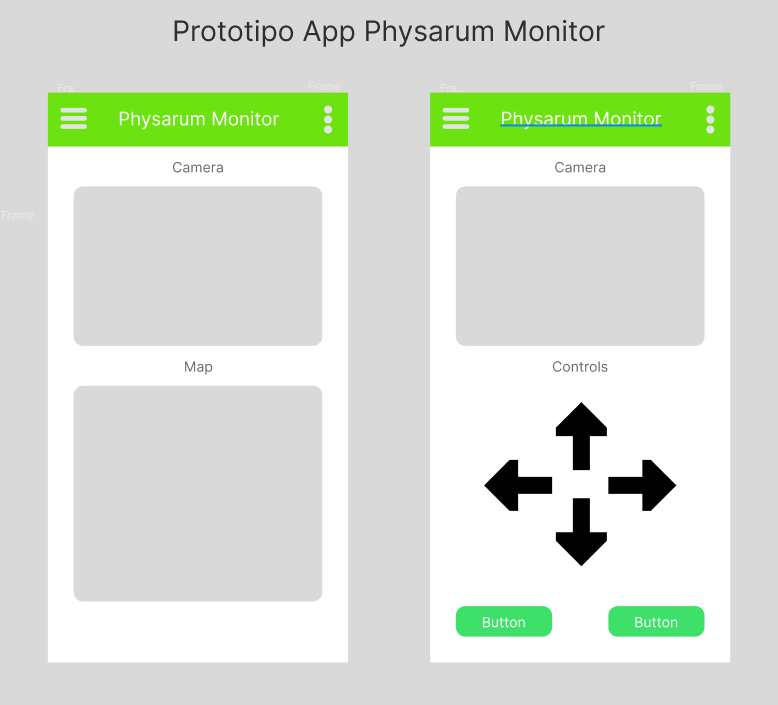
\includegraphics[width=0.5\textwidth]{./images/Pruebas/simulador/image077.png}
        \caption{Prototipo App Physarum Monitor}
        \label{fig:77}
    \end{figure}
    \vskip 0.5cm
    Con la disposici\'on mostrada, podemos ver que se colocan
        los elementos que son necesarios para poder cumplir con
        cada una de las funciones que son necesarias para el control
        y monitoreo del robot. Se muestran dos configuraciones, una
        de las cuales contiene tanto la vista de la c\'amara, as\'i como
        de la vista de la informaci\'on que se nos es enviada por parte
        del robot, la cual es obtenida con el sensor LiDAR. La
        siguiente configuraci\'on contiene tanto la vista de la c\'amara
        del robot, como una serie de botones los cuales representan
        cada uno de los movimientos con los cuales es posible
        controlar al robot. Esta configuraci\'on en particular est\'a
        dise\~nada para poder observar por medio de la c\'amara los
        movimientos que se est\'an realizando a trav\'es de los botones
        y as\'i, tener una mejor noci\'on de lo que se est\'a haciendo con
        el robot, as\'i como para poder orientarse y poder tener un
        mejor control de este robot.